% 欧姆定律微分形式
% Author: ldc
\documentclass[tikz,border=10pt]{standalone}
\usepackage{unicode-math}
\setmainfont{Arial}
\setmathfont[version=normal]{Arial}
\setmathfont[range=\mathscr]{Latin Modern Math}
\usepackage{tikz}
\usetikzlibrary{calc}
\begin{document}
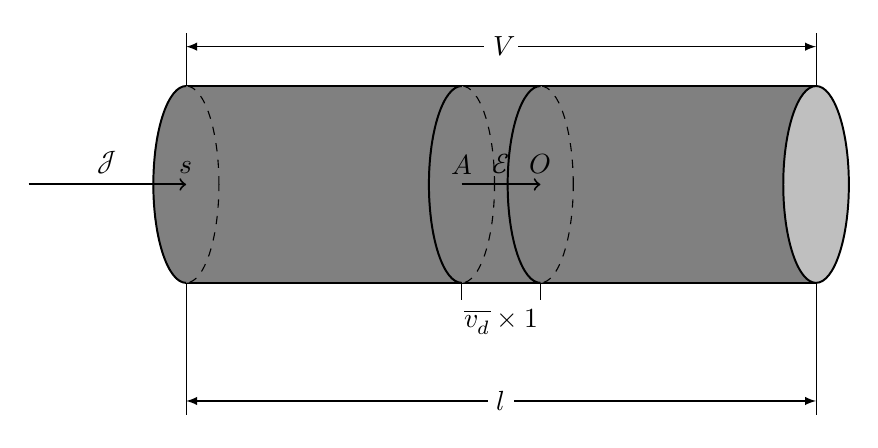
\begin{tikzpicture}
  \def\XSTART{0} %开始圆柱的x坐标
  \def\YSTART{3} %开始圆柱底部的y坐标
  \def\YDIAONE{2.5} %第一个圆柱的直径
  
  \def\GOLONG{1} %电子移动的长度
  \def\XEND{15}
  \def\XONESTART{2}
  \def\XONEDELTA{8} %第一个圆柱的长度
  \def\XTOA{3.5} %A面到最左端的长度
  \def\DD{0.5}
  \def\DDTWO{1.5}
  \def\XA{\XONESTART + \XTOA}
  \def\XO{\XA + \GOLONG}

  \def\YEND{\YSTART+\YDIAONE}
  %\def\XCURVESTART{\XEND/2-\XSTART/2-\XCURVE/2}
  %\def\XCURVESTARTUP{\XEND/2-\XSTART/2-\XCURVE}
  %\def\XCURVEEND{\XEND/2-\XSTART/2 + \XCURVE/2}
  \def\XONEEND{\XONESTART+\XONEDELTA} %第一个圆柱结束的x坐标
  \def\XTWOSTART{\XONEEND+\GOLONG} %第二个圆柱的开始x坐标
  \def\XTWODELTA{3} %第二个圆柱的长度
  \def\XTWOEND{\XTWOSTART+\XTWODELTA} %第二个圆柱结束的x坐标
  \def\YTWOMIDDLE{\YSTART+\YDIATWO/2}
  \def\YONEMIDDLE{\YSTART+\YDIAONE/2}
  %\def\GROUND{\YSTART/4}

  \tikzset{
      partial ellipse/.style args={#1:#2:#3}{
          insert path={+ (#1:#3) arc (#1:#2:#3)}
      },
      dimen/.style={<->,>=latex,thin,
        every rectangle node/.style={fill=white,midway}},
  }

  \draw [line width=0.25mm, fill=gray] (\XONESTART,\YSTART) coordinate (BA)
    rectangle (\XONEEND,{\YSTART+\YDIAONE}) coordinate (BB);
  \draw [line width=0.25mm, fill=lightgray](\XONEEND,\YONEMIDDLE) 
    ellipse ({\YDIAONE/6} and {\YDIAONE/2});
  \draw [fill=gray,dashed](\XONESTART,\YONEMIDDLE)
    ellipse ({\YDIAONE/6} and {\YDIAONE/2});
  \draw [line width=0.25mm](\XONESTART,\YONEMIDDLE)node [above] {$s$}
    [partial ellipse=90:270:{\YDIAONE/6} and {\YDIAONE/2}];
  \draw [fill=gray,dashed]({\XONESTART+\XTOA},\YONEMIDDLE)
    ellipse ({\YDIAONE/6} and {\YDIAONE/2});
  \draw[line width=0.25mm] ({\XONESTART+\XTOA},\YONEMIDDLE)node [above] {$A$}
    [partial ellipse=90:270:{\YDIAONE/6} and {\YDIAONE/2}];
  \draw [fill=gray,dashed]({\XONESTART+\XTOA+\GOLONG},\YONEMIDDLE)
    ellipse ({\YDIAONE/6} and {\YDIAONE/2});
  \draw [line width=0.25mm]({\XONESTART+\XTOA+\GOLONG},\YONEMIDDLE)node [above] {$O$}
    [partial ellipse=90:270:{\YDIAONE/6} and {\YDIAONE/2}];

	
  %\draw [fill=gray] (0,0) rectangle  (\XEND,\GROUND);

  \draw ($(BA)+(0,\YDIAONE)$) -- ++(0,\DD) coordinate (D1) -- +(0,5pt);
  \draw (BB) -- ++(0,\DD) coordinate (D2) -- +(0,5pt);
  \draw [dimen] (D1) -- (D2) node {$V$};
  
  \draw (BA) -- ++(0,-\DDTWO) coordinate (D3) -- +(0,-5pt);
  \draw ($(BB)-(0,\YDIAONE)$) -- ++(0,-\DDTWO) coordinate (D4) -- +(0,-5pt);
  \draw [dimen] (D3) -- (D4) node {$l$};
  
  \draw (\XA,\YSTART) -- ++(0,-\DD) coordinate (D5) -- +(0,-5pt);
  \draw (\XO,\YSTART) -- ++(0,-\DD) coordinate (D6) -- +(0,-5pt);
  \draw [dimen] (D5) -- (D6) node {$\overline{v_d}\times 1$};

  \draw ($(BA)!0.5!(BB)$) -- ++(5pt,0) coordinate (E) -- +(5pt,0);
  \draw [line width=0.25mm, style=->](\XSTART,\YONEMIDDLE) -- (\XONESTART,\YONEMIDDLE)
    node [midway,above] {$\mathcal{J}$};
  
  %\draw ($(BA)!0.5!(BB)$) -- ++(5pt,0) coordinate (E) -- +(5pt,0);
  \draw [line width=0.25mm, style=->](\XA,\YONEMIDDLE) -- (\XO,\YONEMIDDLE)
   node [midway,above] {$\mathscr{E}$};

\end{tikzpicture}
\end{document}